%!TEX root = ../template.tex
%%%%%%%%%%%%%%%%%%%%%%%%%%%%%%%%%%%%%%%%%%%%%%%%%%%%%%%%%%%%%%%%%%%%
%% chapter3.tex
%% NOVA thesis document file
%%
%% Chapter with a short latex tutorial and examples
%%%%%%%%%%%%%%%%%%%%%%%%%%%%%%%%%%%%%%%%%%%%%%%%%%%%%%%%%%%%%%%%%%%%

\typeout{NT FILE chapter3.tex}%

% \makeatletter
% \newcommand{\ntifpkgloaded}{%
%   \@ifpackageloaded%
% }
% \makeatother


\chapter{Planning}
\label{cha:Planning}

\section{Time Scheduling}

    To plan the dissertation it is necessary to create a timeline with the tasks defined and the intervals that must be completed, as shown in Figure \ref{fig:TimelineScheduling}. The developed plan is based on preliminary ideas and information about the thesis. It is not final and may be modified to correct the project's development.

    The timeline described in Figure \ref{fig:TimelineScheduling} presents only a high level of the timeline, while Figures \ref{fig:CollectionProcessing} - \ref{fig:TestsConclusionWriting} depict the sub-tasks.

    \begin{figure}[htbp]
        \centering
        \fboxsep=0pt\fboxrule=0.5pt
        \rotatebox{90}{\fbox{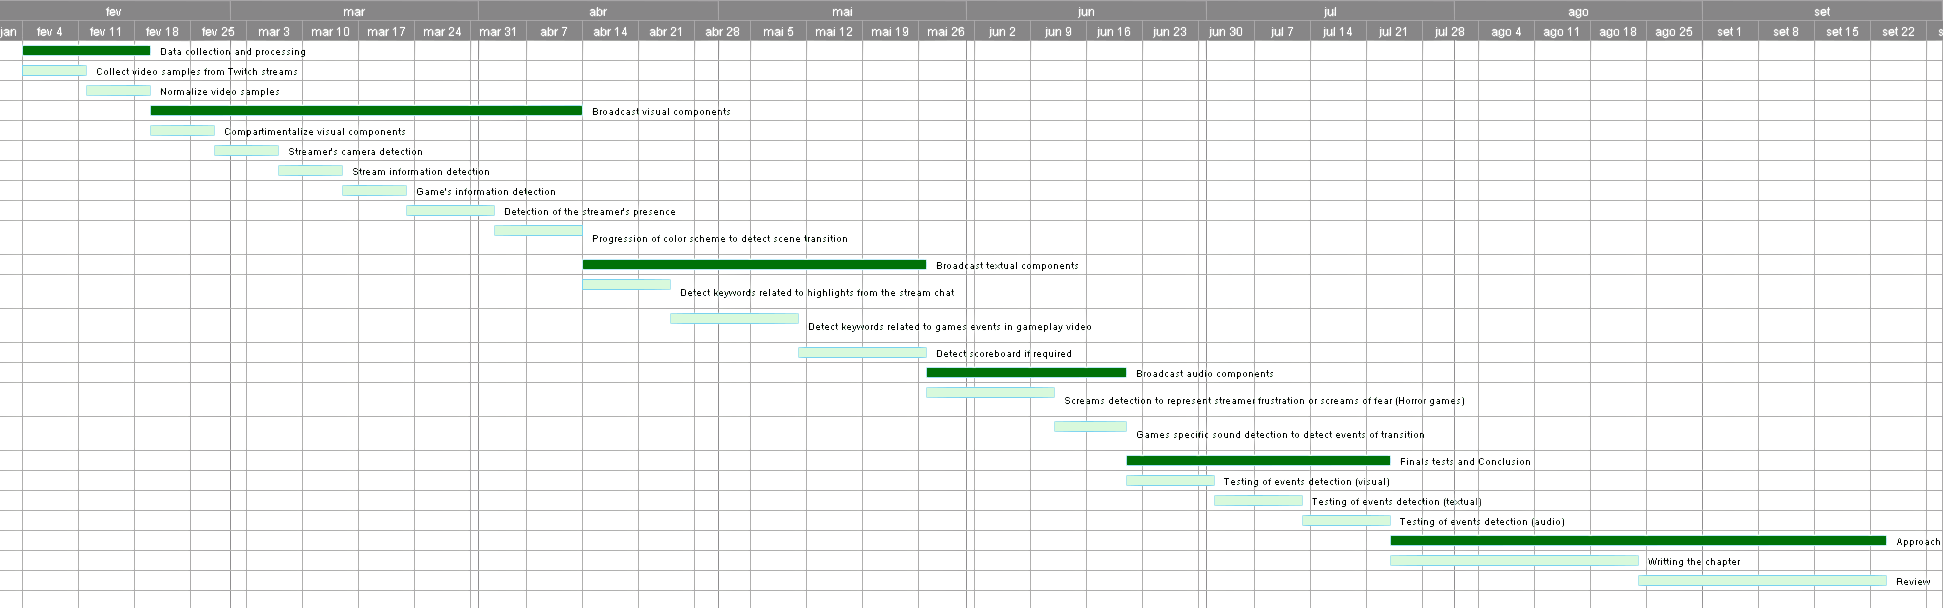
\includegraphics[height=2.8in]{Chapters/Figures/TaskSheet}}}%
        \caption{Proposed timeline to the development}
        \label{fig:TimelineScheduling}
    \end{figure}

    \begin{figure}[htbp]
        \centering
        \fboxsep=0pt\fboxrule=0.5pt
        {\fbox{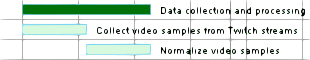
\includegraphics[width=\linewidth]{Chapters/Figures/Data collection and processing}}}%
        \caption{Task of data collection and processing}
        \label{fig:CollectionProcessing}
    \end{figure}

    \begin{figure}[htbp]
        \centering
        \fboxsep=0pt\fboxrule=0.5pt
        {\fbox{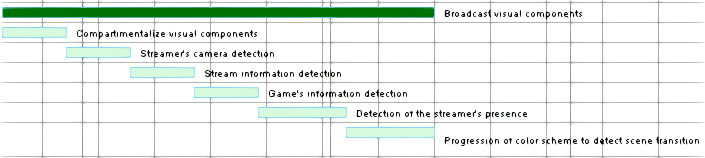
\includegraphics[width=\linewidth]{Chapters/Figures/Broadcast visual component}}}%
        \caption{Task of detection of visual components of the broadcast}
        \label{fig:BroadcastVisualComponents}
    \end{figure}

    \begin{figure}[htbp]
        \centering
        \fboxsep=0pt\fboxrule=0.5pt
        {\fbox{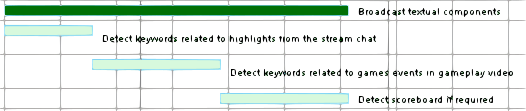
\includegraphics[width=\linewidth]{Chapters/Figures/Broadcast textual components}}}%
        \caption{Task of detection of textual components of the broadcast}
        \label{fig:BroadcastTextualComponents}
    \end{figure}

    \begin{figure}[htbp]
        \centering
        \fboxsep=0pt\fboxrule=0.5pt
        {\fbox{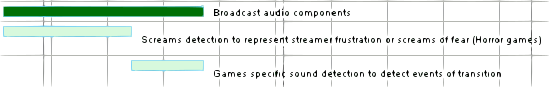
\includegraphics[width=\linewidth]{Chapters/Figures/Broadcast audio components}}}%
        \caption{Task of detection of audio components of the broadcast}
        \label{fig:BroadcastAudioComponents}
    \end{figure}

    \begin{figure}[htbp]
        \centering
        \fboxsep=0pt\fboxrule=0.5pt
        {\fbox{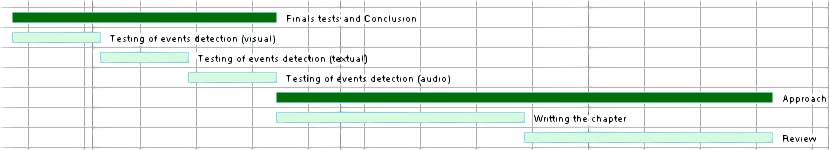
\includegraphics[width=\linewidth]{Chapters/Figures/TestsConclusionsWritting}}}%
        \caption{Task of testing the system and Writing the dissertation}
        \label{fig:TestsConclusionWriting}
    \end{figure}

    The first task (Figure \ref{fig:CollectionProcessing}) to be done for the development of the system is to collect multiple video samples from Twitch streams. These samples will then be normalized to a unique format. Following these normalizations, it is needed to divide the broadcast videos into various visual components to facilitate the process of \gls{LLF}s (Figure \ref{fig:BroadcastVisualComponents}). From the chat of the stream, it is possible to extract information about the interactions between the streamer and viewers or between viewers and other viewers. This task consists of collecting those textual \gls{LLF}s and processing it to a higher level of understanding (Figure \ref{fig:BroadcastTextualComponents}). From the gameplay video, it's possible to infer scenario changes, game information, and much more to detect events that portray the game streamed. The audio component of the stream contains information about the spoken interaction between the streamer and viewer as well as the reactions of the streamer to the game (Figure \ref{fig:BroadcastAudioComponents}). After the development of the system, it is required to test it against the results previewed. These results will be necessary to conclude the efficiency of the development and the practicability of it. All of these developments and testing will then be described and evaluated in the written dissertation (Figure \ref{fig:TestsConclusionWriting}).

    

    

    